\documentclass[12pt,letterpaper,twoside]{article}
\usepackage[left=2cm,right=2cm,top=2cm,bottom=2cm]{geometry}
\usepackage[spanish]{babel}
%\usepackage[fixlanguage]{babelbib}
\usepackage{amsmath,amsfonts,amssymb,float}
\usepackage{kpfonts}
\usepackage{multicol}
\usepackage{enumitem}
\usepackage{authblk}
\usepackage{indentfirst}

%\usepackage[numbers]{natbib}

\usepackage[utf8]{inputenc}
\usepackage{mathrsfs}
\usepackage{fancyhdr,helvet}
\usepackage{units}
\usepackage{physics}
\usepackage{tikz}
\usepackage{caption}
\parindent=12.5pt
\decimalpoint

\newcommand{\helv}{\fontfamily{phv}\fontsize{9}{11}\selectfont}

\pagestyle{fancy}
\renewcommand{\sectionmark}[1]{\markright{\thesection\ #1}}
\fancyhf{}
\fancyfoot[LE,RO]{\helv\thepage}
\fancyhead[LO]{\helv\rightmark} 
\fancyhead[RE]{\helv J. Arias, F. Serrano}

\usepackage{graphicx}
\usepackage{xcolor}

%\AtBeginDocument{\renewcommand\contentsname{Contenidos}}
\AtBeginDocument{\renewcommand\refname{Bibliografía}}  
\AtBeginDocument{\renewcommand\figurename{Figura}}  
\AtBeginDocument{\renewcommand\tablename{Cuadro}}  

\providecommand{\keywords}[1]{\textbf{\textit{Palabras clave:}} #1}

\title{Simulación numérica de la serie del actínido en GNU Octave con ecuaciones diferenciales estocásticas}

\author[$\dagger$]{J. Arias}
\author[$*$]{F. Serrano}

\affil[$\dagger$]{\small Escuela de Física, Facultad de Ciencias, Universidad Nacional Autónoma de Honduras.\newline \textcolor{blue}{jmarias@unah.hn}}
\affil[$*$]{\small Instituto de Investigación en Energía, Universidad Nacional Autónoma de Honduras.}
\date{\today}

\begin{document}
\maketitle

        \begin{abstract}

\noindent Los elementos conocidos en la naturaleza muestran variaciones en su estructura nuclear. De especial interés son los radioisótopos; estos son átomos de un elemento que difieren del resto de su especie por el número de neutrones en su núcleo o por el nivel energético del mismo y que se desintegran hasta obtener una estructura estable. El uranio-235 es un radioisótopo natural. Su desintegración se suscita mediante una reacción en cadena en la que cada producto de fisión es inestable y se descompone en otro elemento en su debido turno. El modelo matemático que describe la reacción en cadena del U-235, también llamada serie del actínido, es las ecuaciones de Bateman. Para que la reacción en cadena tome lugar se requiere una masa mínima de material fisionable conocida como masa crítica. En cada proceso de desintegración se libera una cantidad de energía que puede transformarse en electricidad. Utilizamos GNU Octave para simular la serie del actínido mediante los métodos de Euler-Maruyama, Runge-Kutta y Monte Carlo. 
  
    \end{abstract}
    \keywords{Desintegración en cadena, serie del actínido, ecuaciones de Bateman, simulación numérica}

    \begin{center}
    \textbf{Objetivos}
\end{center}\vspace{-0.5cm}

\textbf{Objetivo general:}
\begin{itemize}
    \item Simular numéricamente en GNU Octave la desintegración en cadena
 del uranio-235.
\end{itemize}

\textbf{Objetivos particulares:}
\begin{itemize}
    \item Resolver completamente las ecuaciones de Bateman para la serie
 del actínido mediante los métodos de Euler-Maruyama, Runge-Kutta y Monte Carlo.
    \item Obtener una comparación de la eficiencia computacional de los métodos elegidos.
\end{itemize}
    \newpage
    \begin{center}
        \section*{Introducción} 
        \addcontentsline{toc}{section}{Introducción}
        \input{introduction}
    \end{center}

\begin{multicols}{2}
    
    \section{Reacciones nucleares}
        Las reacciones nucleares —aquellas en las que participan los núcleos atómicos—, explica \cite{Murray.2020}, pueden tener lugar espontáneamente o inducirse. Estas reacciones son mucho más energéticas que las químicas, pero obedecen a las mismas leyes físicas, continúa \cite{Murray.2020}. 

La literatura clasifica las reacciones nucleares en dos grupos principales: reacciones de fisión y reacciones de fusión, como se puede revisar en \cite{Basdevant.2005, Cottingham.2001, Krane.1987, Murray.2020} entre otros.

\subsection{Reacciones de Fisión}
La fisión nuclear es la ruptura de un núcleo espontáneamente o inducida, de acuerdo con \cite{Basdevant.2005}, en la cual un núcleo pesado se convierte en un sistema de fragmentos más livianos \cite{Murray.2020}. Tal ruptura implica una liberación de energía hacia el entorno, razón por la cual se identifica esta reacción como exotérmica \cite{Basdevant.2005, Murray.2020}. 

Las sustancias radiactivas requieren de un volumen menor de materia que una fuente de combustibles fósiles para generar una cantidad equivalente de energía, de acuerdo con \cite{Sanctis.2016}. 

La mínima cantidad de materia requerida para sustentar una reacción en cadena para una muestra radiactiva cuyos productos se mantienen inestables se llama \textit{masa crítica}, y su estimación es un problema central en física nuclear aplicada como lo muestra \cite{MoralesBolio.1974}. 

\subsection{Reacciones de Fusión}
La fusión nuclear, en palabras de \cite{Murray.2020} es la combinación de dos o más núcleos atómicos en uno más pesado. Estas reacciones también se manifiestan como exotérmicas, en particular, la energía solar que recibe nuestro planeta es esencialmente producida por este fenómeno, explica \cite{Basdevant.2005}. 
\iffalse
\subsection{Energía de desintegración}
Siguiendo la notación empleada en \cite{Krane.1987}, una reacción nuclear general se puede expresar como:
\begin{equation*}
  a + X \longrightarrow Y + b  
\end{equation*}
$X$ e $Y$ representan núcleos atómicos, mientras que $a$ y $b$ son partículas que interceden en la reacción ya sea induciendo el proceso o siendo generadas por el proceso. La ley de la conservación de la energía dicta, en el régimen relativista, la siguiente correspondencia entre el antes y el después del proceso nuclear:

\begin{equation*}
    m_Xc^2+T_x+m_ac^2+T_a\ = m_Yc^2+T_Y+m_bc^2+T_b,
\end{equation*}

\noindent donde T representa la energía cinética de las partículas. Las emes, $m_X,\ m_a,\ m_Y,\ m_b$, representan las masas de las partículas en cuestión. Se define el valor Q (energía de la reacción o energía de desintegración) como:
\begin{equation*}
    Q=(m_{inicial}-m_{final})c^2,  
\end{equation*}
\noindent o como el exceso de la energía final de los productos.
\begin{equation*}
   Q=T_{final}-T_{inicial}
\end{equation*}    
\fi
    
    \section{Modos de desintegración nuclear}
        De acuerdo con \cite{Sanctis.2016} y \cite{Podgorsak.2016}, se debe entender el proceso mediante el cual un núcleo atómico se separa en fragmentos más pequeños sin un estímulo externo como un proceso de radiactividad. Bajo este mismo razonamiento se dice que el núcleo atómico es radiactivo y que atraviesa una desintegración o decaimiento radiactivo. 

Suele identificarse al núcleo original como núcleo padre \cite{Sanctis.2016, Podgorsak.2016} y sus productos de desintegración se les identifica como hijos o partículas hijas\cite{Podgorsak.2016, Sanctis.2016}. 

La radiactividad se cuantifica en términos de \textit{actividad} y su unidad SI es el becquerel ($\unit{Bq}$), \cite{Podgorsak.2016}. 
\subsection{Leyes de la desintegración nuclear}

\noindent Siguiendo a \cite{Krane.1987}, las leyes de la desintegración radiactiva son: 
\begin{enumerate}
	\item Existe la misma probabilidad de que todos los núcleos de un elemento radiactivo se desintegran. 
	
	\item La tasa de desintegración espontánea de un elemento radiactivo es proporcional al número de núcleos presentes en ese momento.
	
\end{enumerate}

\noindent Matemáticamente, y en concordancia con \cite{Podgorsak.2016}, se puede escribir un modelo para la ley de desintegración radiactiva como: 

\begin{equation*}
\dv{N}{t} \propto N
\end{equation*}

\noindent donde $N$ es el número de átomos presentes en el tiempo $t$. Dicha proporción se traduce en la siguiente ecuación: 

\begin{equation}
\dv{N}{t} = -\lambda N\label{ecuaciondiferencialN}
\end{equation} 

\noindent donde $\lambda $ es la constante de decaimiento del elemento y dicta una propiedad intrínseca del material independiente de su condición química o física, explica \cite{Sanctis.2016} y \cite{Podgorsak.2016}. El signo negativo indica que a medida que el tiempo $t$ aumenta, el número de núcleos $N$ disminuye. La ecuación \ref{ecuaciondiferencialN} puede resolverse mediante variable separable, notando que

\begin{equation}
\frac{\dd{N}}{N} = -\lambda \dd{t},
\end{equation} 

\noindent de integrar esto se obtiene: 

\begin{equation}
\ln( \lambda ) = -\lambda t + C\label{ecuacionlambda}
\end{equation}

\noindent donde C es una constante de integración y se evalúa por el hecho de que en t = 0 el número de átomos del elemento radiactivo es $N_0$. Debido a esta condición inicial se establece que 

\begin{equation*}
C = \ln(N_0)
\end{equation*}

Se sigue que 

\begin{equation*}
ln\left( \frac{N}{N_0} \right) = - \lambda t,
\end{equation*}

\noindent la cual es equivalente a

\begin{equation*}
N(t) = N_0 \exp(- \lambda t)
\end{equation*}

\noindent La relación de $N$ a $t$ se ha representado gráficamente en la figura \ref{decaimientodelsodio24} en los anexos para $ ^{24} Na$, radioisótopo del sodio que presenta un período de semidesintegración $t_{1/2} = 15h$.

\subsection{Canales de decaimiento}

Siguiendo a \cite{Cottingham.2001, Basdevant.2005, Krane.1987} los canales de desintegración (o \textit{decaimiento}) son los posibles mecanismos en que una partícula puede fraccionarse, estos se muestran en la figura \ref{channels} documentada en anexos.

\noindent La desintegración radiactiva se produce a través de la emisión de diferentes tipos de radiaciones corpusculares, explican \cite{Krane.1987, Podgorsak.2016, Sanctis.2016}. Los principales son: 

\begin{itemize}
	\item Radiación alfa ($\alpha $):  la partícula emitida corresponde a un núcleo de helio. La masa del nuevo núcleo disminuye en cuatro unidades, con relación al núcleo inicial. 
	
	\item Radiación beta ($\beta $): la partícula emitida es un electrón o un anti-electrón como consecuencia de la transmutación de un neutrón en protón, o al revés. El número atómico de masa permanece igual. Un neutrino  se lleva la energía complementaria liberada en la transformación. 
	
	\item Radiación gamma ($\gamma $): es un tipo de radiación electromagnética que transporta el exceso de energía de un núcleo inestable o metaestable. 
\end{itemize}

Los diversos modos de desintegración de un núcleo radiactivo son catalogados de acuerdo con la emisión del núcleo atómico:

\begin{itemize}
	\item Decaimiento Alfa:
	
	En este proceso, el núcleo padre se desintegra para dar un núcleo hijo y una partícula $\alpha$ ($^{4} He$). 
	
	\item Decaimiento Beta:
	
	En este proceso, el núcleo padre se desintegra para dar un núcleo hijo y una partícula $\beta $. La desintegración $\beta $ se subdivide en tres categorías, cuya descripción se sigue de la discusión desarrollada en \cite{Cottingham.2001, Krane.1987, Das.2009, Martin.2009}: 
	
    \begin{itemize}
    	\item \textbf{Emisión de electrones o $\beta^{-}$}: al desintegrarse el núcleo padre una partícula $\beta ^{-}$ y un anti-neutrino son expulsados. El número de masa del núcleo hijo es igual al del padre y el número atómico es mayor que el del padre por una unidad. 
    	
    	\item \textbf{Emisión de anti-electrones o $\beta^{+}$}: al decaer el núcleo padre una partícula $\beta^{+}$ y un neutrino son expulsados. El número de masa del núcleo hijo es el mismo que el del padre y el número atómico es una unidad menor que el del padre. 
    	
    	\item \textbf{Captura de electrones}: el núcleo padre captura uno de los electrones orbitales emitiendo un neutrino. El número de masa del núcleo hijo es igual al del padre, pero su número atómico disminuye en una unidad. 
 	\end{itemize}
 
	\item Decaimiento Gamma: las desintegraciones alfa y beta de un núcleo radiactivo pueden dejar al núcleo hijo en un estado excitado. Esta energía excedente puede puede perderse en forma de radiaciones electromagnéticas, llamadas rayos g. Dichos rayos pueden ser absorbidos por electrones orbitales y dar lugar a una creación de pares electrón-antielectrón.
\end{itemize}

La constante de decaimiento juega un rol importante en la comprensión de radiactividad. Pues, de acuerdo con \cite{Sanctis.2016} y \cite{Podgorsak.2016} este parámetro da una medida de probabilidad bien definida para la desintegración por unidad de tiempo de un isótopo radiactivo.

El recíproco de la constante de decaimiento, $\tau_{1/2}$, se conoce como período de semidesintegración y se reporta en unidades de tiempo (años, días, horas o segundos) \cite{Podgorsak.2016}. 

Cualquiera de esos dos parámetros permite no solo caracterizar una entidad radiactividad, pero también sus modos de desintegración. 

\subsection{Desintegración en cadena}
No es raro el evento en la naturaleza en que un núcleo inestable produce hijos inestables que continúan desintegrándose a su propio ritmo, \cite{Podgorsak.2016} identifica estos procesos como \textit{reacciones en cadena} o \textit{cadenas de desintegración}. 

Para \cite{Sanctis.2016} una secuencia de procesos de decaimiento define una \textit{familia radiactiva}, estos son radioisótopos que toman parte en la secuencia o cadena. 

Muchas familias de decaimiento son estudiadas y explotadas con diversos fines, ver \cite{Eidemuller.2021} y \cite{Koizumi.2021}. Una de especial interés es la desintegración el uranio-235 llamada también serie del actínido \cite{Krane.1987}.

En estos procesos secuenciales se pueda dar una acumulación de núcleos en donde la tasa de decaimiento de un núcleo alcanza a la de otros. En \cite{Sanctis.2016}, \cite{Podgorsak.2016} y \cite{Krane.1987} se discute suficientemente las condiciones de equilibrio y sus instancias así como la ley de radiactividad en el contexto de acumulación de núcleos. La serie del actínido no es la excepción a este modelo, como se verá más adelante.  

En una cadena de desintegración no todos los hijos se desintegran por el mismo canal, algunos núcleos incluso presentan bifurcaciones en su proceso de fisión con una probabilidad de decaer por un canal u otro, se dice que la secuencia se ramifica\cite{HUBENER2003211, Cottingham.2001, Podgorsak.2016} y a la probabilidad de decaer por un canal u otro se le llama tasa de ramificación \cite{Sanctis.2016} o fracción de ramificación \cite{Podgorsak.2016}.

\subsection{Ecuaciones de Bateman}
\noindent Las ecuaciones de Bateman son un sistema de ecuaciones diferenciales ordinarias propuestas por el matemático británico Harry Bateman en 1910 para generalizar las cadenas de desintegración del tipo $Padre\rightarrow Hijo \rightarrow Nieto$ \cite{Podgorsak.2016}.

\noindent Debido a que la cantidad de núcleos que participan en el proceso de desintegración es tan grande, podemos suponer que la función $N=N(t)$ que da el número de núcleos en un tiempo $t$ es una función continua, no discreta. De esta manera, es posible aplicar sobre ella las reglas de cálculo como ya las conocemos \cite{Podgorsak.2016}. 

\noindent Siguiendo a \cite{Podgorsak.2016}, la cadena de desintegración descrita en el modelo de Bateman comprende las siguientes condiciones iniciales:

\begin{equation}
    \eval{N_1(t)}_{t=0}=N_1(0)\neq 0,\label{condicioninicialpadre}
\end{equation}
\begin{equation}
    N_2(0)=N_3(0)=...=N_i(0)=0, \label{condicioninicialproductos}
\end{equation}

El significado o la implicación de las ecuaciones \ref{condicioninicialpadre} y \ref{condicioninicialproductos} es que, en un tiempo inicial, $t=0$, únicamente se dispone de los núcleos de la muestra padre para desintegración nuclear, mientras que los productos de su fisión permanecen inexistentes \cite{Podgorsak.2016}. Es solo hasta que el padre ha decaído que los valores de $N$ son distintos de cero para los elementos resultantes de la fisión y los procesos de acumulación \cite{Sanctis.2016} son evidentes. 

El número de núcleos disponibles en un tiempo $t$ para el k-ésimo producto de fisión viene dado por:

\begin{equation}
        N_k(t)=N_1^{(0)} \left[C_1 e^{-\lambda_1 t}+...+C_k e^{-\lambda_k t}\right] \label{iesimonucleo}
\end{equation}

\noindent Donde $N_1^{(0)}$ es el número inicial de núcleos de la muestra radiactiva. Para los valores numéricos de los coeficientes $C_k$ de Bateman, \textit{Flanagan y Senftle} en \cite{Flanagan1954} ofrecen tablas completas de los términos que involucran.

Siguiendo a \cite{Loch.2013}, una generalización más compacta válida para cualquier núcleo en la secuencia está dada como

\begin{equation}
\!\!\small N_m(t)=N_1^{(0)} \prod_{k=1}^{m-1}\!\!\lambda_k\sum_{j=1}^{m}\left(\!\!\frac{e^{\lambda_j t}}{\prod\limits_{p=1, p\neq j}^{m}\left(\lambda_p-\lambda_j\right)}\!\!\right) \label{batemangeneral}
\end{equation}

De acuerdo con \cite{Pratiwi.2021}, Bateman habría resuelto sus ecuaciones con transformadas de Laplace, y este método sería efectivo para sistemas lineales \textit{bien portados}, pero en el caso de reacciones en cadena con bifurcaciones en los productos de desintegración el sistema requiere de un tratamiento matricial numérico. 
       
    \section{Serie del actínido}\label{actinidoserie}
        Como parte del proceso de desintegración radiactiva, los productos de fisión del uranio emiten neutrones y rayos gamma al atravesar una serie de decaimientos beta y alfa, según \cite{Guo.2016}. La causa de esta serie de desintegraciones nucleares se debe a la razón de neutrones sobre protones, explica \cite{Guo.2016}. 

Es sabido que los núcleos pesados muestran una tendencia a la inestabilidad cuando el número de neutrones supera al de protones \cite{Podgorsak.2016, Krane.1987}.  

De acuerdo con \cite{Guo.2016}, al momento de analizar una cadena de desintegración compleja se simplifica el problema al resolver la reacción a través de reacciones lineales en las que cada núcleo está relacionado solo a un núcleo padre. No obstante, es apreciable de inmediato que la naturaleza estocástica del proceso es obviada con esta suposición.

El proceso de desintegración del uranio-235 contempla bifurcaciones en varios puntos, esto es: hay productos de desintegración que pueden a su vez producir uno de dos posibles núcleos más estables como se documenta en \cite{HUBENER2003211, International_Atomic_Energy_Agency2013-bq}. 

En la literatura científica se registran más bifurcaciones o menos para el proceso, en virtud de los valores de las constantes de ramificación, como podemos apreciar en \cite{HUBENER2003211,International_Atomic_Energy_Agency2013-bq,Pratiwi.2021,Loch.2013}. 

Para mantener la simulación lo más fiel posible al proceso real, se ha tomado como referencia la cadena presentada en \cite{HUBENER2003211}, la cual está ilustrada en la imagen \ref{cadenadelu235} replicada para fines de continuidad de la lectura en anexos.

\subsection{Ecuaciones de Bateman para la serie del actínido}
Tomando en cuenta las condiciones iniciales \ref{condicioninicialpadre} y \ref{condicioninicialproductos} y la forma de $N_i(t)$ en \ref{iesimonucleo}, las ecuaciones de Bateman para la serie del actínido son:
\begin{align}
    N_1'(t)&=-\lambda_1 N_1(t)\\ \label{ecubateman1} %Uranio
    N_2'(t)&=\lambda_1 N_1(t) -\lambda_2 N_2(t)\\ %Torio
    N_3'(t)&=\lambda_2 N_2(t) -\lambda_3 N_3(t)\\ %Paladio
    N_4'(t)&=\lambda_3 N_3(t) -\lambda_4 N_4(t)\\ %Actinio
    N_5'(t)&=(1-f_4)\lambda_4 N_4(t) -\lambda_5 N_5(t)\\ %Torio
    N_6'(t)&=f_4 \lambda_4 N_4(t) -\lambda_6 N_6(t)\\ %Francio
    N_7'(t)&=\lambda_5 N_5(t) + \lambda_6 N_6(t) -\lambda_7 N_7(t)\\ %Radio
    N_8'(t)&=\lambda_7 N_7(t) -\lambda_8 N_8(t)\\ %Radón
    N_9'(t)&=\lambda_8 N_8(t) -\lambda_9 N_9(t)\\ %Polonio
    N_{10}'(t)&=f_9\lambda_9 N_9(t) -\lambda_{10} N_{10}(t)\\ %Plomo
    N_{11}'(t)&=(1-f_9)\lambda_9 N_9(t) -\lambda_{10} N_{11}(t)\\%Astato
   N_{12}'(t)&=\lambda_{10} N_{10}(t) +\lambda_{11} N_{11}(t)\\
   &-\lambda_{12} N_{12}(t)\\ %Bismuto
   %\end{align}
   %
   %\begin{align}
    N_{13}'(t)&=(1-f_{12})\lambda_{12} N_{12}(t)\\
    & -\lambda_{13} N_{13}(t)\\ %Polonio
    N_{14}'(t)&=f_{12}\lambda_{12}N_{11}(t) -\lambda_{14} N_{14}(t)\\ %Talio
    N_{15}'(t)&=\lambda_{13} N_{13}(t) + \lambda_{14} N_{14}(t) %Plomo
    \label{ecubateman15}
\end{align}

\noindent donde $f_k$ son tasas de ramificación. Las $N_i(t)$ se definen de la siguiente manera:
\begin{itemize}
    \item $N_1(t)\equiv$ \textit{Núcleos de} $^{235}U$.
    \item $N_2(t)\equiv$ \textit{Núcleos de} $^{231}Th$.
    \item $N_3(t)\equiv$ \textit{Núcleos de} $^{231}Pa$.
    \item $N_4(t)\equiv$ \textit{Núcleos de} $^{227}Ac$.
    \item $N_5(t)\equiv$ \textit{Núcleos de} $^{227}Th$.
    \item $N_6(t)\equiv$ \textit{Núcleos de} $^{223}Fr$.
    \item $N_7(t)\equiv$ \textit{Núcleos de} $^{223}Ra$.
    \item $N_8(t)\equiv$ \textit{Núcleos de} $^{219}Rn$.
    \item $N_9(t)\equiv$ \textit{Núcleos de} $^{215}Po$.
    \item $N_{10}(t)\equiv$ \textit{Núcleos de} $^{211}Pb$
    \item $N_{11}(t)\equiv$ \textit{Núcleos de} $^{215}At$.
    \item $N_{12}(t)\equiv$ \textit{Núcleos de} $^{211}Bi$.
    \item $N_{13}(t)\equiv$ \textit{Núcleos de} $^{211}Po$.
    \item $N_{14}(t)\equiv$ \textit{Núcleos de} $^{207}Tl$.
    \item $N_{15}(t)\equiv$ \textit{Núcleos de} $^{207}Pb$.
\end{itemize}

\noindent para los factores de ramificación tenemos:
\begin{itemize}
    \item $f_4=\frac{\lambda_{4,\alpha}}{\lambda_{4,\alpha}+\lambda_{4,\beta}}$, donde $\lambda_{4,\alpha}$ es la tasa de desintegración del $^{227}Ac$ hacia $^{223}Fr$, mientras que $\lambda_{4,\beta}$ representa la tasa de desintegración de $^{227}Ac$ hacia $^{227}Th$. 
    \item $f_9=\frac{\lambda_{9,\alpha}}{\lambda_{9,\alpha}+\lambda_{9,\beta}}$, donde $\lambda_{9,\alpha}$ es la tasa de desintegración del $^{215}Po$ hacia $^{211}Pb$, mientras que $\lambda_{9,\beta}$ representa la tasa de desintegración de $^{215}Po$ hacia $^{215}At$.
    \item $f_{12}=\frac{\lambda_{12,\alpha}}{\lambda_{12,\alpha}+\lambda_{12,\beta}}$, donde $\lambda_{12,\alpha}$ es la tasa de desintegración del $^{211} Bi$ hacia $^{207} Tl$, mientras que $\lambda_{12,\beta}$ representa la tasa de desintegración de $^{211} Bi$ hacia $^{211} Po$.
\end{itemize}

De acuerdo con los archivos de \textit{National Nuclear Data Center} en la base de datos \textit{NuDat}, las probabilidades para el canal alfa y el beta en el Ac-227 son 0.013800 y 0.98620, respectivamente; para el canal alfa y beta en el Po-215 son, respectivamente, 0.9999977 y 0.0000023; para el canal alfa y el beta en el Bi-211 son 0.99724 y 0.00276, respectivamente.

Entonces $f_4=0.01380$, $f_9=0.9999977$ y $f_{11}=0.99724$.

La constante de decaimiento $\lambda_i$ para el i-ésimo núcleo depende del período de semi-desintegración $\tau_{1/2}^{(i)}$, estos valores son conocidos y están documentados en la literatura, tal es el caso de \cite{Flanagan1954} y la base datos \textit{NuDat}. 

La tabla \ref{tabladeconstantesdedesintegracion} muestra las constantes de decaimiento de cada núcleo en las ecuaciones \ref{ecubateman1} hasta \ref{ecubateman15} junto con el período de semi-desintegración que le concierne según \textit{NuDat}.

Lo que no se muestra en la tabla \ref{tabladeconstantesdedesintegracion} es las constantes de decaimiento correspondientes a los canales específicos $\alpha$ y $\beta$ en la desintegración del $^227 Ac$, $^215 Po$, y $^211 Bi$. De la definición de razón de fraccionamiento, se puede deducir que

$$\lambda_{4,\alpha}=0.4394\times 10^{-3}\unit{a^{-1}}$$
$$\lambda_{4,\beta}=3.140\times 10^{-3}\unit{a^{-1}}$$
$$\lambda_{9,\alpha}=1.227\times 10^{10}\unit{a^{-1}}$$
$$\lambda_{9,\beta}=2.822\times 10^{4}\unit{a^{-1}}$$
$$\lambda_{11,\alpha}=2.180\times 10^{11}\unit{a^{-1}}$$
$$\lambda_{11,\beta}=6.033\times 10^{8}\unit{a^{-1}}$$

\noindent son las constantes de decaimiento que caracterizan los canales de desintegración observados en la serie del actínido. 

Hay que señalar que en este modelo, las ecuaciones de Bateman tienen una forma determinista. Bajo la perspectiva de un modelo estocástico diferencial, vemos que la solución del sistema sería la solución esperada para el caso determinista más un término perturbativo que es en sí una variable aleatoria dependiente del tiempo. 

En la literatura se reportan métodos analíticos para resolver sistemas de ecuaciones como el planteado aquí empleando transformadas de Laplace o exponenciales de matrices. En este ensayo, se emplea el método de eigenvectores para establecer la solución general del sistema. Al notar que el sistema de ecuaciones puede representarse con una ecuación matricial de la forma

\begin{equation}
	\mathbf{N'}(t)=\Lambda \mathbf{N}(t)\label{sistemadinamicoU235}
\end{equation}


\noindent donde $\mathbf{N}(t)$ es un vector cuya iésima componente es la función $N_i(t)$ del iésimo núcleo en la cadena. El vector derivada $\mathbf{N'}(t)$ es el vector que contiene las derivadas de las funciones iésima. La matriz $\Lambda$ de dimensión $15\times15$ se da en la ecuación \ref{matriz_determinista} en los anexos.

La matriz $\Lambda$ cumple con ser una matriz triangular (inferior), y en ese sentido sus eigenvalores son los elementos de la diagonal principal, es inmediato verificar que tales eigenvalores son distintos y reales, bajo estas condiciones \cite{Hirsch.2004} sostiene que la solución de un sistema de la forma de \ref{sistemadinamicoU235} viene dada como combinación lineal de los eigenvectores de $\Lambda$:

$$\mathbf{N}(t)=\sum_{i=1}^{15}\kappa_i e^{-\lambda_i t} \mathbf{V}_{\lambda_i}$$

\noindent Las constantes de integración $\kappa_i$ son determinadas por las condiciones iniciales $\mathbf{N}(0)=\left[N_1^{(0)}\ 0\ 0\ ...\ 0\right]^T$.

\subsubsection{Cálculo de los coeficientes de Bateman}

De acuerdo con la ecuación \ref{batemangeneral}, podemos emplear las constantes de decaimiento en el cuadro \ref{tabladeconstantesdedesintegracion} para determinar los coeficientes de Bateman de la serie del actínido. No obstante, estas soluciones corresponden a los casos donde la serie de desintegración no presenta ramificaciones, la existencia de tales bifurcaciones en el proceso agrega términos sobre la ecuación \ref{batemangeneral} que no están contemplados en esta forma general.

Una solución simbólica de las ecuaciones por medio de Laplace y Laplace Inverso demuestra que las constantes de decaimiento correspondientes a cada ramificación se combinan de forma alternada en las soluciones deterministas de acuerdo con la aparición de estas bifurcaciones en la cadena.

En el método de eigenvectores primero se obtiene una serie de coeficientes de linealización que acompañan a los vectores linealmente independientes que conforman la solución del sistema, estas constantes se resumen en la tabla \ref{tabladecoeficientes2}. 

Multiplicando tales coeficientes con  los vectores solución (eigenvectores) se recuperan los coeficientes de Bateman para esta serie. Se resumen los resultados en los cuadros \ref{tabla_coeficientes_bateman1} al \ref{tabla_coeficientes_bateman4}. Donde $C_k^*=C_k/N_1^{(0)}$ para simplicidad. 

\subsection{Modelo estocástico matricial}
Un modelo estocástico matricial del sistema se puede construir usando una matriz determinista alternativa $\mathcal{L}$ más tres matrices $\mathcal{X}$, $\mathcal{Y}$ y $\mathcal{Z}$ que conjuntamente representan un ruido estocástico sobre $\mathcal{L}$. El sistema matricial es

\begin{equation}
	\mathcal{N}'(t)=(\mathcal{L}+x\mathcal{X}+y\mathcal{Y}+z\mathcal{Z})\mathcal{N}(t)
\end{equation}

\noindent donde los parámetros $x, y,\textrm{ y }z$ son variables aleatorias discretas que pueden ser 0 o 1, no necesariamente todas a las vez, y dictan la ocurrencia de una bifurcación en la cadena. La forma explícita de estos cuatro arreglos puede verse en los anexos en las ecuaciones \ref{matriz_determinista_alternativa}, \ref{matriz_estocastica_x}, \ref{matriz_estocastica_y} y \ref{matriz_estocastica_z}. El vector $\mathcal{N}$ corresponde al vector de funciones del número de núcleos por unidad de tiempo para cada especie química en la cadena bajo el esquema estocástico. 

    \section{Implementación en GNU Octave}
        \subsection{Método de Runge-Kutta Estocástico}

\subsection{Método de Euler-Maruyama}

\subsection{Monte Carlo}
        
    \section{Análisis y discusión de los resultados}
        \input{section5_analisis_discusion}

    \section{Conclusiones}
        \input{conclusion}

\end{multicols}
    \section{Anexos}
        \subsection{Matrices del sistema}
La matriz $\Lambda$ de coeficientes de desintegración del sistema es un arreglo disperso. A continuación se muestra dejando en blanco aquellos elementos valuados en 0:

\begin{equation}
	\Lambda=\left(\begin{smallmatrix}
		-\lambda_1& & & & & & & & & & & & & & \\
		 \lambda_1&-\lambda_2& & & & & & & & & & & & & \\
		 & \lambda_2&-\lambda_3& & & & & & & & & & & & \\
		 & & \lambda_3&-\lambda_4& & & & & & & & & & & \\
		 & & &\lambda_{4,\beta}&-\lambda_5& & & & & & & & & & \\
		 & & &\lambda_{4, \alpha}& &-\lambda_6& & & & & & & & & \\
		 & & & & \lambda_5& \lambda_6&-\lambda_7& & & & & & & & \\
		 & & & & & & \lambda_7&-\lambda_8& & & & & & & \\
		 & & & & & & & \lambda_8&-\lambda_9& & & & & & \\
		 & & & & & & & &\lambda_{9,\alpha}&-\lambda_{10}& & & & & \\
		 & & & & & & & &\lambda_{9, \beta}& &-\lambda_{11}& & & & \\
		 & & & & & & & & & \lambda_{10}&\lambda_{11}&-\lambda_{12}& & & \\
		 & & & & & & & & & & &\lambda_{12, \beta}&-\lambda_{13}& & \\
		 & & & & & & & & & & &\lambda_{12, \alpha}& &-\lambda_{14}& \\ 
		 & & & & & & & & & & & &\lambda_{13}&\lambda_{14}& 0\\
	\end{smallmatrix}\right)
\end{equation}\label{matriz_determinista}

Para la versión estocástica del sistema, se toma como término determinista la matriz $\mathcal{L}$ y las matrices estocásticas $\mathcal{X}$, $\mathcal{Y}$ y $\mathcal{Z}$ dadas por los siguientes arreglos dispersos:

\begin{equation}
	\mathcal{L}=\left(\begin{smallmatrix}
		-\lambda_1& & & & & & & & & & & \\								%fila 1
		\lambda_1&-\lambda_2& & & & & & & & & & \\						%fila 2
		&\lambda_2&-\lambda_3& & & & & & & & & \\						%fila 3
		& & \lambda_3&-\lambda_4& & & & & & & & \\						%fila 4
		& & &\lambda_{4, \alpha}&-\lambda_6& & & & & & & \\				%fila 5
		& & & &\lambda_6 &-\lambda_7& & & & & & \\						%fila 6
		& & & & &\lambda_7&-\lambda_8& & & & & \\						%fila 7
		& & & & & &\lambda_8&-\lambda_9& & & & \\						%fila 8
		& & & & & & &\lambda_{9, \beta}&-\lambda_{11}& & & \\			%fila 9
		& & & & & & & &\lambda{11}&-\lambda_{12}& & \\					%fila 10
		& & & & & & & & &\lambda_{12, \beta}&-\lambda_{14}&\\			%fila 11 
		& & & & & & & & & &\lambda{14}& 0\\								%fila 12
	\end{smallmatrix}\right)
\end{equation}\label{matriz_determinista_alternativa}

\begin{equation}
	\mathcal{X}=\begin{cases}
		(\lambda_4-2\lambda_{4, \alpha}) & \textrm{En la fila 5, columna 4.}\\
		-\lambda_5+\lambda_6 & \textrm{En la fila 5, columna 5.}\\
		\lambda_5-\lambda_6 & \textrm{En la fila 6, columna 5.}
	\end{cases}
\end{equation}\label{matriz_estocastica_x}

\begin{equation}
	\mathcal{Y}=\begin{cases}
		-(\lambda_9-2\lambda_{9, \alpha}) & \textrm{En la fila 9, columna 8.}\\
		-\lambda_{10}+\lambda_{11} & \textrm{En la fila 9, columna 9.} \\
		\lambda_{10}-\lambda_{11} & \textrm{En la fila 10, columna 9.} \\
	\end{cases}
\end{equation}\label{matriz_estocastica_y}

\begin{equation}
	\mathcal{Z}=\begin{cases}
		(\lambda_{12}-2\lambda_{12, \alpha}) & \textrm{En la fila 11, columna 10.}\\
		-\lambda_{13}+\lambda_{14} & \textrm{En la fila 11, columna 11.}\\
		\lambda_{13}-\lambda_{14}  & \textrm{En la fila 12, columna 11.}\\
	\end{cases}
\end{equation}\label{matriz_estocastica_z}

\noindent donde se suponen 0 todos los elementos no especificados.

\subsection{Tablas de coeficientes}
A continuación se presentan los coeficientes obtenidos para la serie del actínido mediante la simulación por GNU Octave bajo el esquema de eigenvectores. 
\begin{center}
\begin{tabular}[h]{|c|r|r|r|r|}
    \hline
    $N_i$ & $C_1^*$ & $C_2^*$ & $C_3^*$ & $C_4^*$  \\\hline\hline
    $N_1$ & $1.00000000$ & $0$ & $0$ & $0$ \\
    $N_2$ & $5.51288098\times 10^{-7}$& $-5.51288098\times 10^{-7}$ & $0$ & $0$ \\
    $N_3$ & $4.65333818\times 10^{-5}$& $5.57897907\times 10^{-7}$ & $-4.70912797\times 10^{-5}$ & $0$ \\
    $N_4$ & $3.09248238\times 10^{-8}$& $3.92796956\times 10^{-10}$ & $-3.13163987\times 10^{-8}$ & $-1.22207337\times 10^{-12}$ \\
    $N_5$ & $1.00429565\times 10^{-12}$& $1.27579176\times 10^{-14}$ & $-1.01701378\times 10^{-12}$ & $-3.97809227\times 10^{-17}$ \\
    $N_6$ & $5.86387844\times 10^{-14}$& $7.44810663\times 10^{-16}$ & $-5.93812778\times 10^{-14}$ & $-2.31726572\times 10^{-18}$ \\
    $N_7$ & $4.44937366\times 10^{-11}$& $5.65191533\times 10^{-13}$ & $-4.50571672\times 10^{-11}$ & $-1.76087766\times 10^{-15}$ \\
    $N_8$ & $1.78377969\times 10^{-16}$& $2.26588562\times 10^{-18}$ & $-1.80636795\times 10^{-16}$ & $-7.05946067\times 10^{-21}$ \\
    $N_9$ & $8.02482795\times 10^{-20}$& $1.01937152\times 10^{-21}$ & $-8.12644752 \times 10^{-20}$ & $-3.17589429 \times 10^{-24}$ \\
    $N_{10}$ & $9.75861373\times 10^{-14}$& $1.23960972\times 10^{-15}$ & $-9.88218850\times 10^{-14}$ & $-3.86206702\times 10^{-18}$ \\
    $N_{11}$ & $1.03599574\times 10^{-26}$& $1.31599652\times 10^{-28}$ & $-1.04911471\times 10^{-26}$ & $-4.10004175\times 10^{-31}$ \\
    $N_{12}$ & $5.78523143\times 10^{-15}$& $7.34881961\times 10^{-17}$ & $-5.85849067\times 10^{-15}$ & $-2.28956247\times 10^{-19}$ \\
    $N_{13}$ & $2.31805658\times 10^{-17}$& $2.94456320\times 10^{-19}$ & $-2.34741047\times 10^{-17}$ & $-9.17393781\times 10^{-22}$ \\
    $N_{14}$ & $3.55803094\times 10^{-17}$& $4.51966849 \times 10^{-19}$ & $-3.60308682\times 10^{-17}$ & $-1.40812647\times 10^{-21}$ \\
    $N_{15}$ & $-1.00004712$& $-7.00318644\times 10^{-9}$ & $4.71226424\times 10^{-5}$ & $1.22388044\times 10^{-12}$ \\
    \hline
\end{tabular}
\captionof{table}{Coeficientes de Bateman obtenidos mediante eigenvectores. Parte 1}\label{tabla_coeficientes_bateman1}
\end{center}

\begin{center}
\begin{tabular}[h]{|c|r|r|r|r|}
    \hline
   $N_i$ & $C_5^*$ & $C_6^*$ & $C_7^*$ & $C_8^*$  \\\hline\hline
   $N_1$ & $0$& $0$ & $0$ & $0$ \\
   $N_2$ & $0$& $0$ & $0$ & $0$ \\
   $N_3$ & $0$& $0$ & $0$ & $0$ \\
   $N_4$ & $0$& $0$ & $0$ & $0$ \\
   $N_5$ & $0$& $4.88856388\times 10^{-25}$ & $0$ & $0$ \\
   $N_6$ & $9.50138278\times 10^{-30}$ & $0$ & $0$ & $0$ \\
   $N_7$ & $-9.51409697\times 10^{-30}$ & $7.69096154\times 10^{-25}$ & $4.78609631\times 10^{-24}$ & $0$ \\
   $N_8$ & $-3.82573383\times 10^{-35}$ & $3.08335862\times 10^{-30}$ & $1.91878144\times 10^{-29}$ & $1.90321436\times 10^{-32}$ \\
   $N_9$ & $-1.72111485\times 10^{-38}$ & $1.38713444\times 10^{-33}$ & $8.63217083\times 10^{-33}$ & $8.56599161\times 10^{-36}$ \\
   $N_{10}$ & $3.26399237\times 10^{-32}$ & $1.68909355\times 10^{-27}$ & $1.05202483\times 10^{-26}$ & $-1.90755340\times 10^{-32}$ \\
   $N_{11}$ & $-2.22193897\times 10^{-45}$ & $1.79077407\times 10^{-40}$ & $1.11440298\times 10^{-39}$ & $1.10588725\times 10^{-42}$ \\
   $N_{12}$ & $2.14355861\times 10^{-33}$ & $1.00143055\times 10^{-28}$ & $6.23756480\times 10^{-28}$ & $3.59322574\times 10^{-35}$ \\
   $N_{13}$ & $8.59228100\times 10^{-36}$ & $4.01258523\times 10^{-31}$ & $2.49930117\times 10^{-30}$ & $1.65548072\times 10^{-37}$ \\
   $N_{14}$ & $1.68328476\times 10^{-35}$ & $6.16008576\times 10^{-31}$ & $3.83733666\times 10^{-30}$ & $-3.10073991\times 10^{-39}$ \\
   $N_{15}$ & $-2.20564442\times 10^{-32}$& $-1.25974588\times 10^{-24}$ & $-4.79726585\times 10^{-24}$ & $-1.27035860\times 10^{-36}$ \\
        \hline
\end{tabular}
\captionof{table}{Coeficientes de Bateman obtenidos mediante mediante eigenvectores. Parte 2}\label{tabla_coeficientes_bateman2}
\end{center}

\begin{center}
	\begin{tabular}[h]{|c|r|r|r|r|}
		\hline
		$N_i$ & $C_9^*$ & $C_{10}^*$ & $C_{11}^*$ & $C_{12}^*$  \\\hline\hline
		$N_1$ & $0$& $0$ & $0$ & $0$ \\
		$N_2$ & $0$& $0$ & $0$ & $0$ \\
		$N_3$ & $0$& $0$ & $0$ & $0$ \\
		$N_4$ & $0$& $0$ & $0$ & $0$ \\
		$N_5$ & $0$& $0$ & $0$ & $0$ \\
		$N_6$ & $0$ & $0$ & $0$ & $0$ \\
		$N_7$ & $0$ & $0$ & $0$ & $0$ \\
		$N_8$ & $0$ & $0$ & $0$ & $0$ \\
		$N_9$ & $-2.88467470\times 10^{-35}$ & $0$ & $0$ & $0$ \\
		$N_{10}$ & $2.88467044\times 10^{-35}$ & $0$ & $-2.17703376\times 10^{-29}$ & $0$ \\
		$N_{11}$ & $-3.94554377\times 10^{-42}$ & $3.04250308\times 10^{-42}$ & $0$ & $0$ \\
		$N_{12}$ & $4.65721718\times 10^{-41}$ & $-3.04250545\times 10^{-42}$ & $-1.37194870\times 10^{-30}$ & $-1.08392039\times 10^{-30}$ \\
		$N_{13}$ & $-6.46462136\times 10^{-46}$ & $2.36278724\times 10^{-48}$ & $-5.49850503\times 10^{-33}$ & $-4.36062925\times 10^{-33}$ \\
		$N_{14}$ & $-1.78300791\times 10^{-48}$ & $6.53807648\times 10^{-51}$ & $-9.72206436\times 10^{-33}$ & $5.4271346\times 10^{-33}$ \\
		$N_{15}$ & $2.23180703\times 10^{-48}$ & $-4.57859868\times 10^{-52}$ & $2.31575069\times 10^{-29}$ & $1.08285388\times 10^{-30}$ \\
		\hline
	\end{tabular}
	\captionof{table}{Coeficientes de Bateman obtenidos mediante mediante eigenvectores. Parte 3}\label{tabla_coeficientes_bateman3}
\end{center}

\begin{center}
	\begin{tabular}[h]{|c|r|r|r|}
		\hline
		$N_i$ & $C_{13}^*$ & $C_{14}^*$ & $C_{15}^*$ \\\hline\hline
		$N_1$ & $0$& $0$ & $0$ \\
		$N_2$ & $0$& $0$ & $0$ \\
		$N_3$ & $0$& $0$ & $0$ \\
		$N_4$ & $0$& $0$ & $0$ \\
		$N_5$ & $0$& $0$ & $0$ \\
		$N_6$ & $0$ & $0$ & $0$ \\
		$N_7$ & $0$ & $0$ & $0$ \\
		$N_8$ & $0$ & $0$ & $0$ \\
		$N_9$ & $0$ & $0$ & $0$ \\
		$N_{10}$ & $0$ & $0$ & $0$ \\
		$N_{11}$ & $0$ & $0$ & $0$ \\
		$N_{12}$ & $0$ & $0$ & $0$ \\
		$N_{13}$ & $4.76594956\times 10^{-34}$ & $0$ & $0$ \\
		$N_{14}$ & $0$ & $-1.20997671\times 10^{-32}$ & $0$ \\
		$N_{15}$ & $-4.76594956\times 10^{-34}$& $1.20997671\times 10^{-32}$ & $1.00000000$ \\
		\hline
	\end{tabular}
	\captionof{table}{Coeficientes de Bateman obtenidos mediante mediante eigenvectores. Parte 4}\label{tabla_coeficientes_bateman4}
\end{center}

\subsection{Gráficas de las soluciones del sistema}
Se presentan las gráficas de las soluciones generadas por Octave en el marco de eigenvectores. 

\begin{figure}[H]
	\centering
	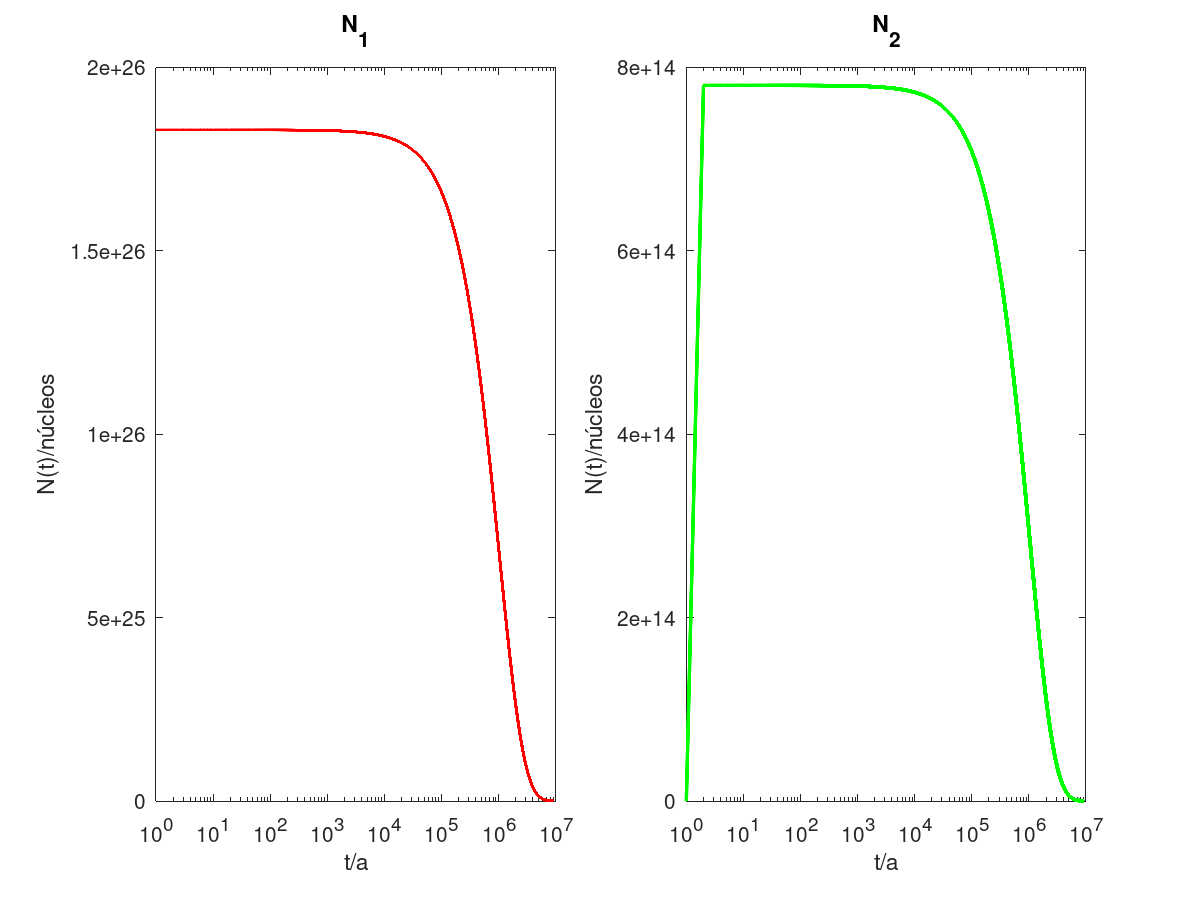
\includegraphics[scale=0.33]{/home/arias/Desktop/Research/u235_decay_chain_numsim/figuras/n1_n2.png}\label{n1n2}\caption{Curvas de desintegración de los núcleos $N_1$ y $N_2$ generadas por GNU Octave.}
\end{figure}

\begin{figure}[H]
	\centering
	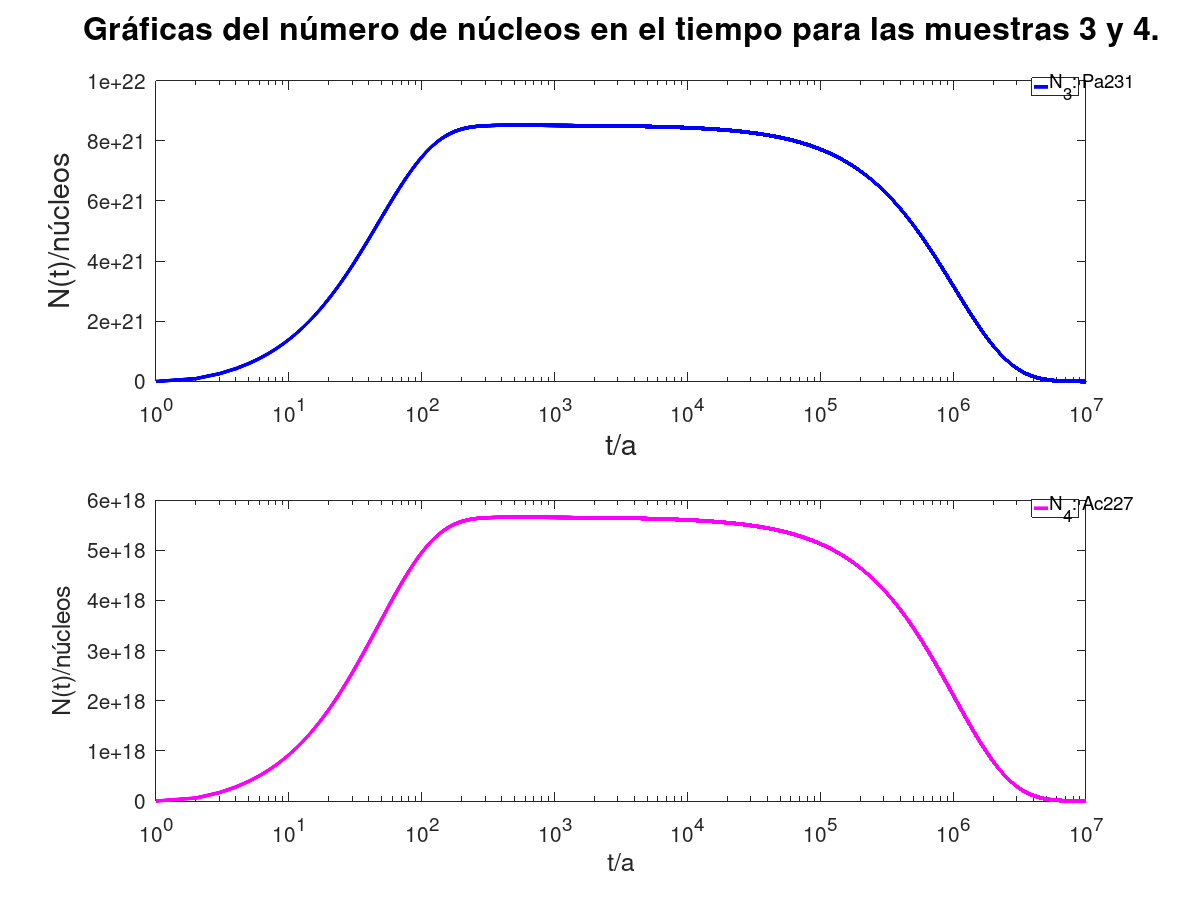
\includegraphics[scale=0.33]{/home/arias/Desktop/Research/u235_decay_chain_numsim/figuras/n3_n4.png}\label{n3n4}\caption{Curvas de desintegración de los núcleos $N_3$ y $N_4$ generadas por GNU Octave.}
\end{figure}

\begin{figure}[H]
	\centering
	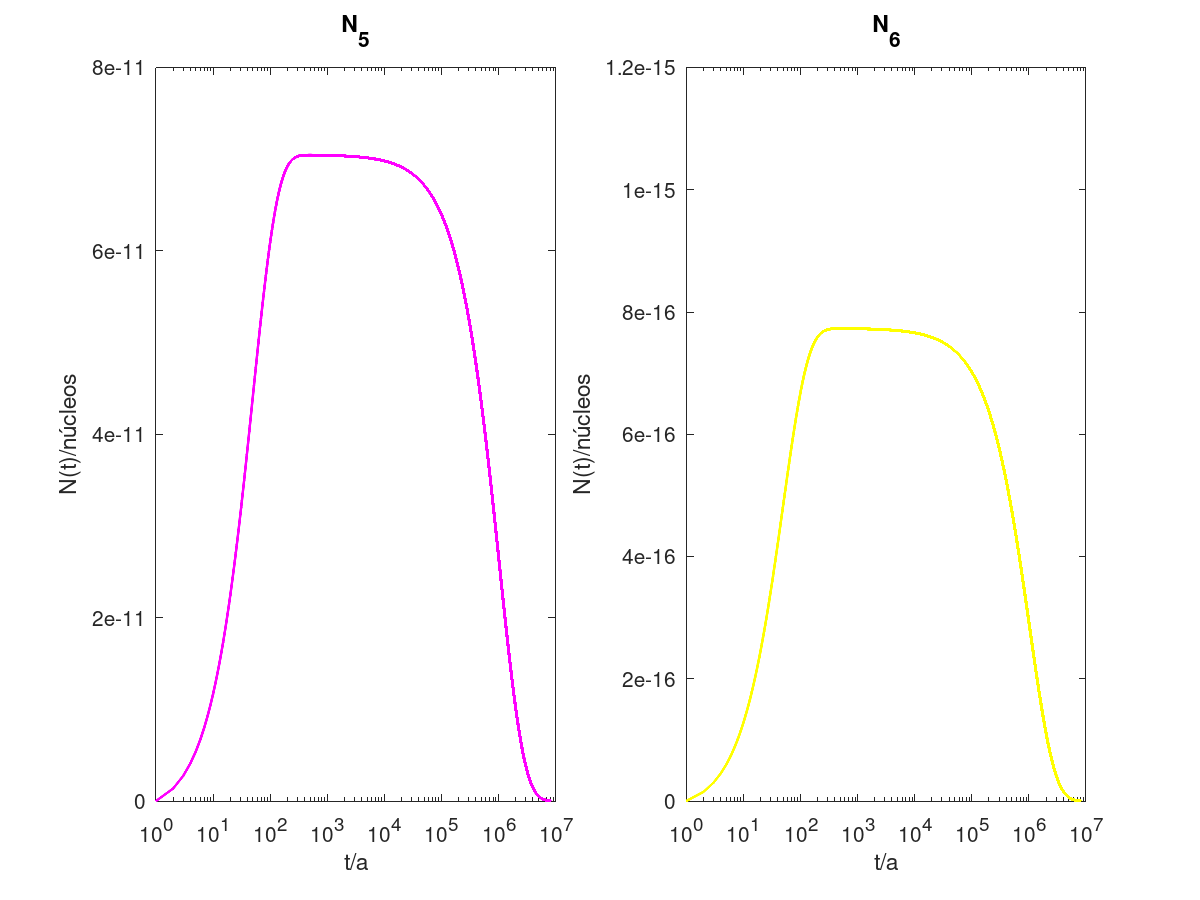
\includegraphics[scale=0.33]{/home/arias/Desktop/Research/u235_decay_chain_numsim/figuras/n5_n6.png}\label{n5n6}\caption{Curvas de desintegración de los núcleos $N_5$ y $N_6$ generadas por GNU Octave.}
\end{figure}

\begin{figure}[H]
	\centering
	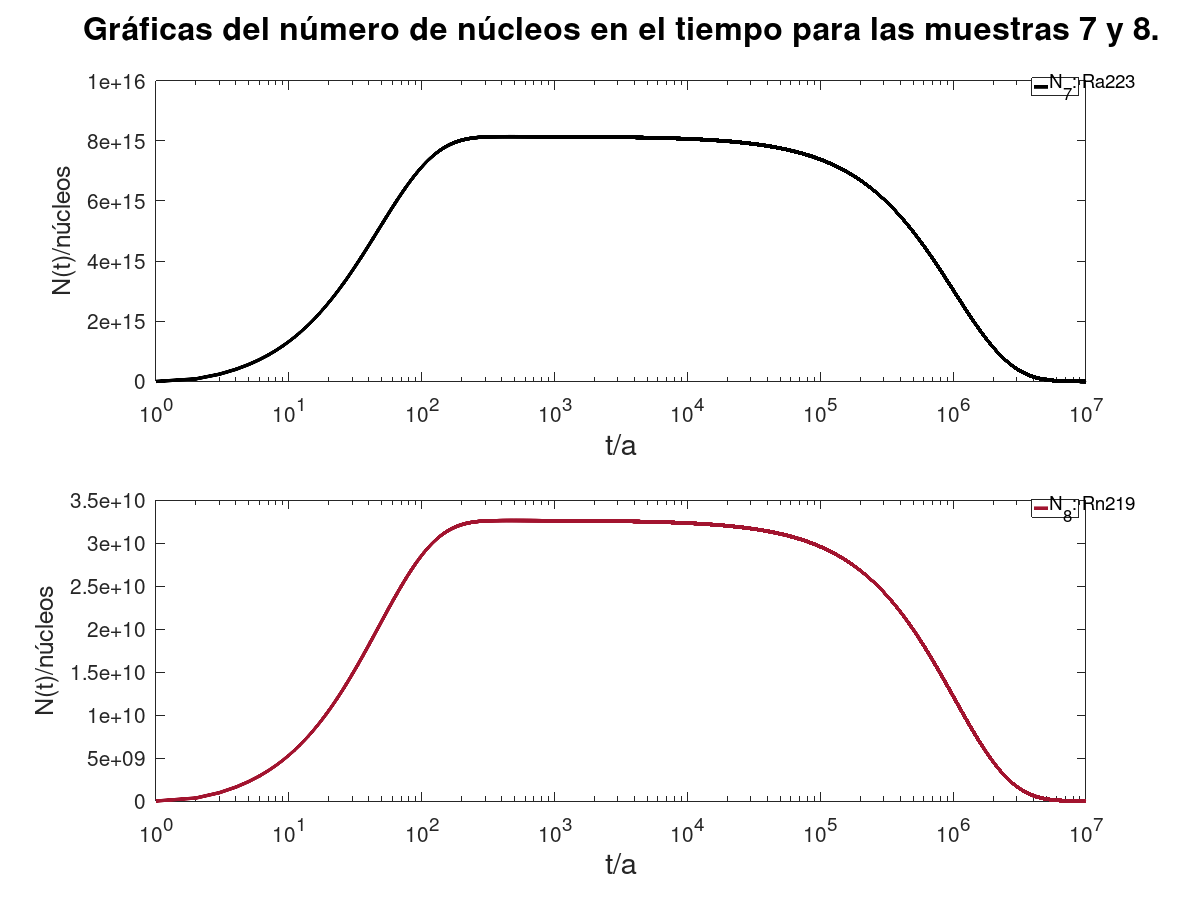
\includegraphics[scale=0.33]{/home/arias/Desktop/Research/u235_decay_chain_numsim/figuras/n7_n8.png}\label{n3n4}\caption{Curvas de desintegración de los núcleos $N_7$ y $N_8$ generadas por GNU Octave.}
\end{figure}

\begin{figure}[H]
	\centering
	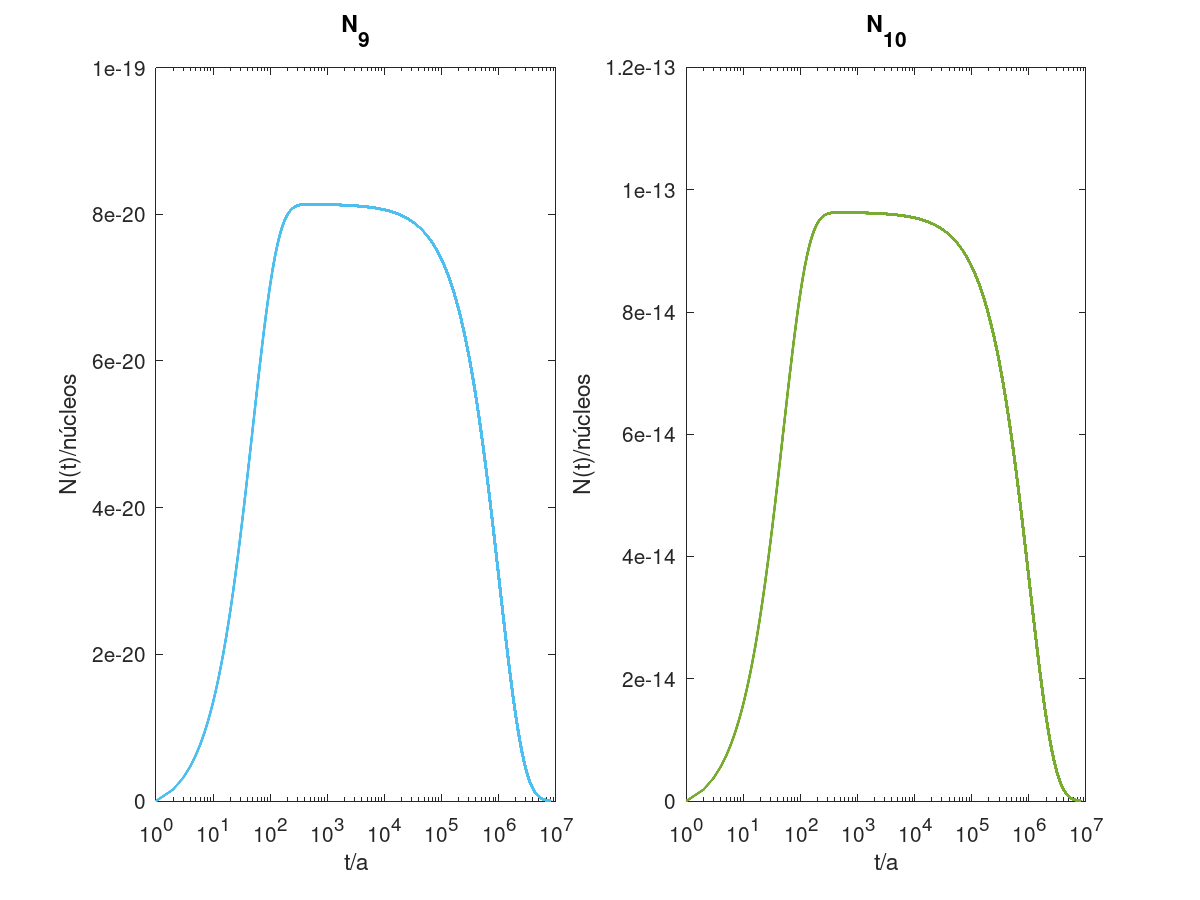
\includegraphics[scale=0.33]{/home/arias/Desktop/Research/u235_decay_chain_numsim/figuras/n9_n10.png}\label{n3n4}\caption{Curvas de desintegración de los núcleos $N_9$ y $N_{10}$ generadas por GNU Octave.}
\end{figure}

\begin{figure}[H]
	\centering
	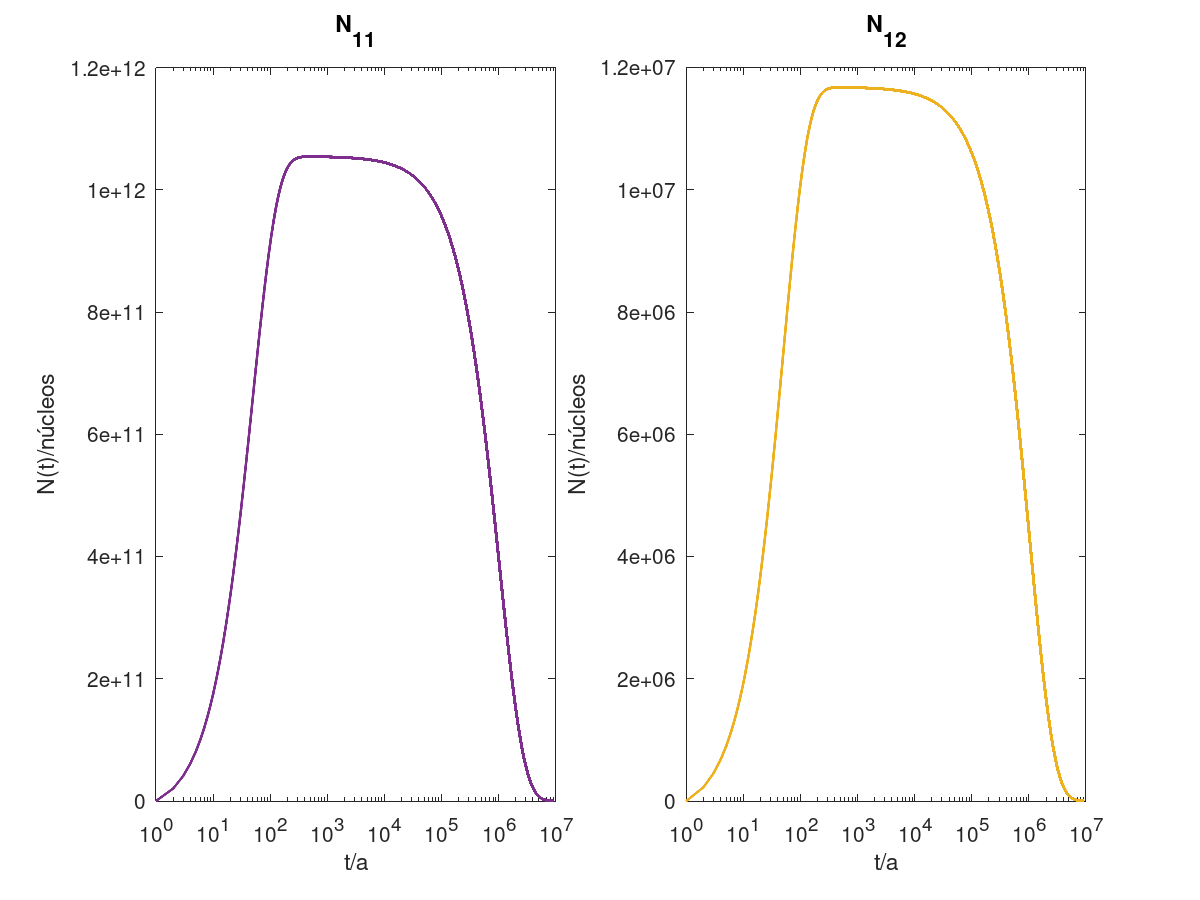
\includegraphics[scale=0.33]{/home/arias/Desktop/Research/u235_decay_chain_numsim/figuras/n11_n12.png}\label{n3n4}\caption{Curvas de desintegración de los núcleos $N_{11}$ y $N_{12}$ generadas por GNU Octave.}
\end{figure}

\begin{figure}[H]
	\centering
	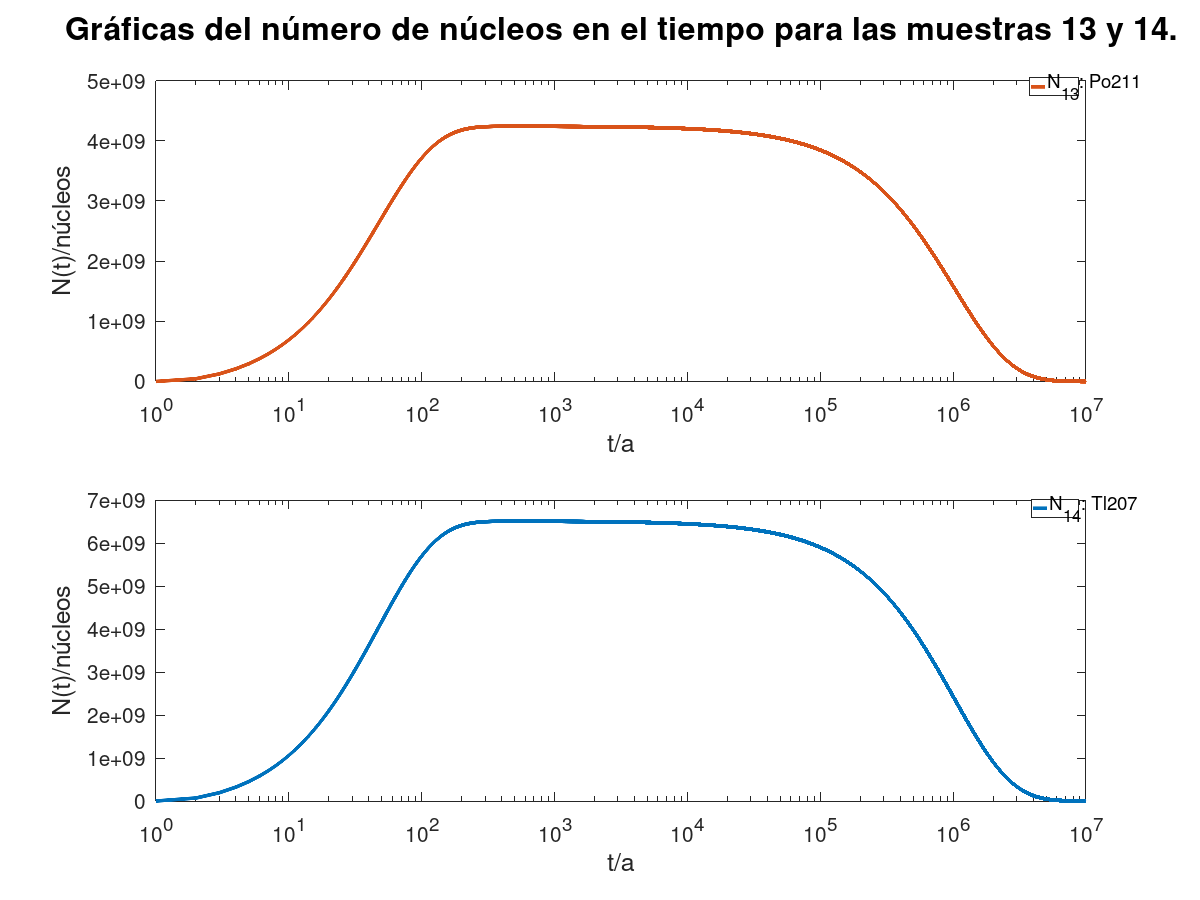
\includegraphics[scale=0.33]{/home/arias/Desktop/Research/u235_decay_chain_numsim/figuras/n13_n14.png}\label{n3n4}\caption{Curvas de desintegración de los núcleos $N_{13}$ y $N_{14}$ generadas por GNU Octave.}
\end{figure}

\begin{figure}[H]
	\centering
	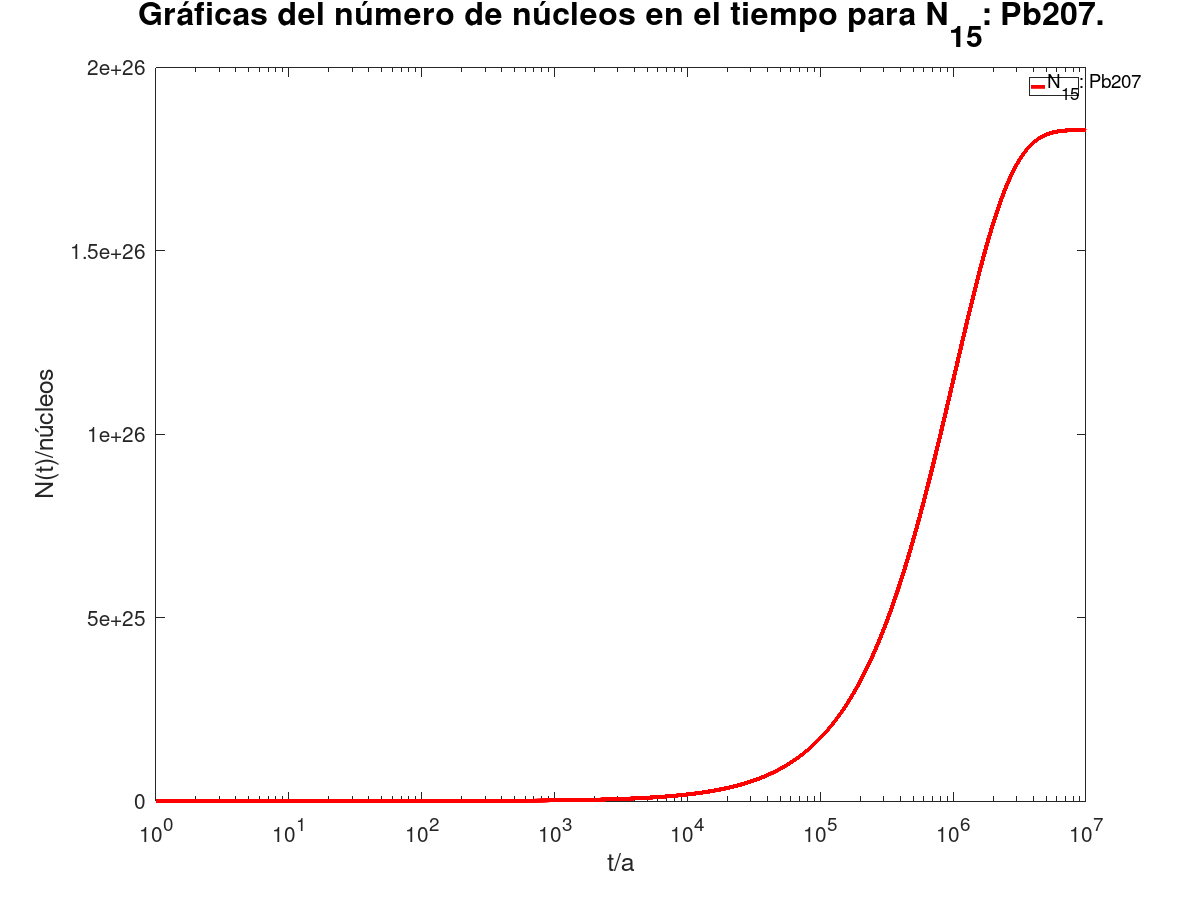
\includegraphics[scale=0.33]{/home/arias/Desktop/Research/u235_decay_chain_numsim/figuras/n15.png}\label{n15}\caption{Curva de desintegración del núcleo $N_{15}$ generada por GNU Octave.}
\end{figure}

\newpage

\bibliographystyle{ieeetr}
\bibliography{proyecto_iie_energia_nuclear.bib}

\end{document}
